%!TEX program = xelatex
%!TEX root = ./thesis.tex

\section{Experiments on the Basic Task \textit{move0}}\label{sec_exp_move0}

The methods for solving the basic task move0 are discussed in this section.

First, we would like to verify the ability to reproducing consistent learning performance discussed in~\cite{henderson2017matters}. We choose the ACKTR~\cite{wu2017scalable} method and test it on the move0 task. As is discussed previously, the move0 task is actually a single-modal environment since the image observation is redundant. Separate neural network parameters are used for the actor network and critic network. The neural networks have the same architecture that consists of two fully connected layers with 64 hidden units after the motion sensor input. The neural network outputs the mean parameter of the policy distribution. The standard deviation of the policy distribution is parameterized by an independent parameter vector. The batch-size is set to 8000, the KL-divergence set to 0.0001 and 20 parallel agents are used to generate experience. The resulting learning performance is shown in Figure~\ref{fig_acktr_reprod}. It appears that the performance of one experiment gets stuck at a score below 3000 while another continues to improve after reaching the score of 4000. 
\begin{figure}[!htbp]
	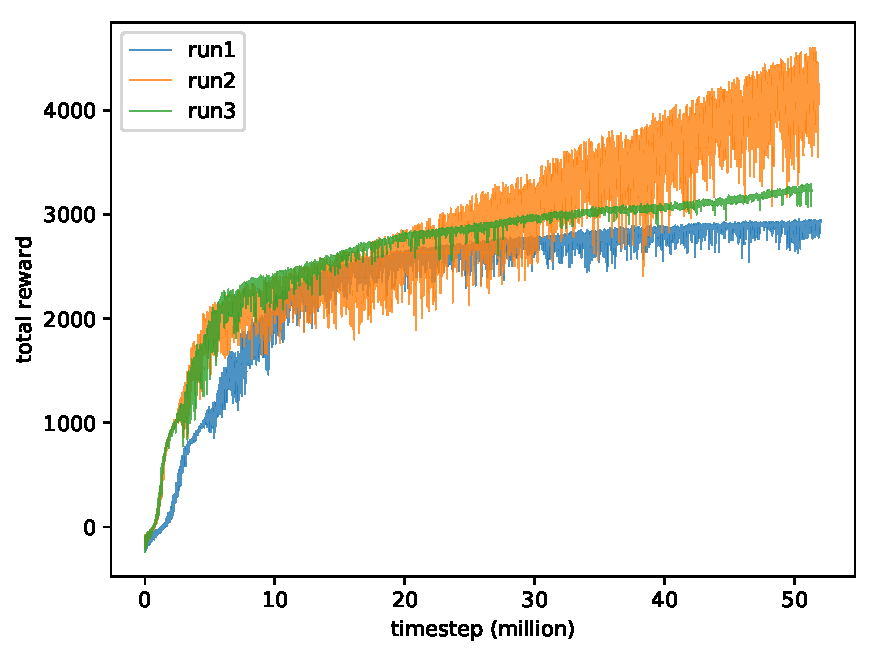
\includegraphics[width=0.7\textwidth]{images/rec_0403_reprod}
	\centering
	\caption{Inconsistent performance produced by ACKTR agents with the same  parameters but different runs. The vertical axis is the total return averaged over the recent 20 episodes and the horizontal axis is the number of million time-steps}\label{fig_acktr_reprod}
\end{figure}

We'd also like to compare the learning performance of the ACKTR method across different learning rates. The experiment result showing the performance of the original ACKTR algorithm with different learning rates is shown in Figure~\ref{fig_acktr_mom_tune}. The result shows that the agents are likely to get stuck at the score of around 3000. 
%The reason might be that while the KL-divergence based trust-region method provides a theoretical guarantee on the monotonic improvement of performance, the agent might converge too early at local minimums and fails to make efficient exploration.
\begin{figure}[!htbp]
	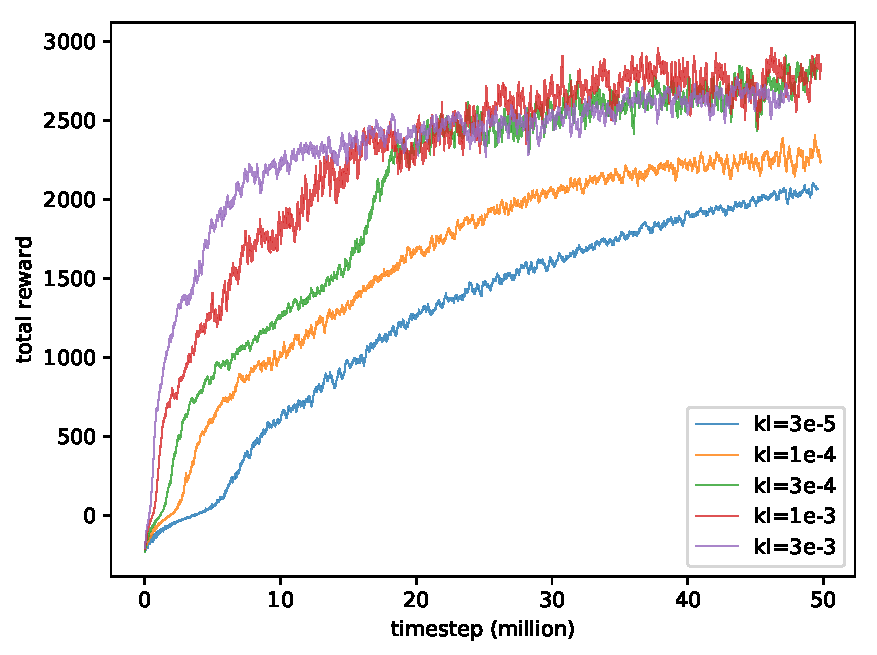
\includegraphics[width=0.7\textwidth]{rec_180521_acktr_mom}
	\centering
	\caption{Performance of ACKTR agents with different KL-divergence constraints. All the agents are trained with batch-size 4000 and 20 parallel agents. The vertical axis is the total return averaged over the recent 200 episodes and the horizontal axis is the number of million time-steps}\label{fig_acktr_mom_tune}
\end{figure}

We'd also like to verify if the proposed W-KTR method is less prone to local minimums on the task move0. The experiment results comparing the performance of W-KTR agents with different learning rates is shown in Figure~\ref{fig_wass_const_tune}. The result shows that none of the W-KTR agents gets stuck at the local minimum around 3000, and their final performance can reach a total return of around 6000. However, the W-KTR agent appears to have a much slower rate of improvement on the performance before 50 million time-steps.
\begin{figure}[!htbp]
	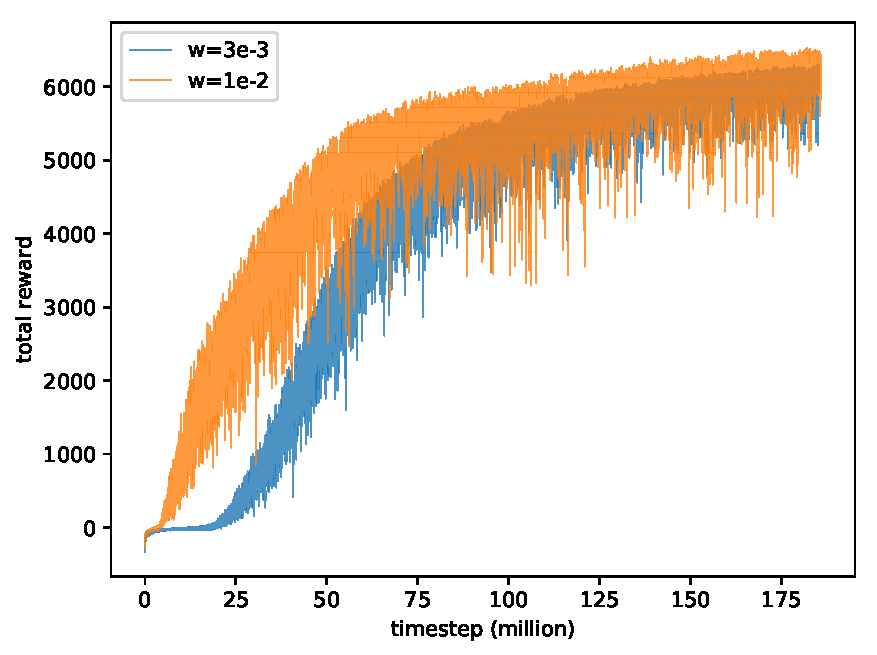
\includegraphics[width=0.7\textwidth]{rec_180608_wass_const}
	\centering
	\caption{Performance of W-KTR agents with different W2-metric constraints. All the agents are trained with batch-size 4000 and 20 parallel agents. The vertical axis is the total return averaged over the recent 20 episodes and the horizontal axis is the number of million time-steps}\label{fig_wass_const_tune}
\end{figure}

We also test if applying a decaying Wasserstein constraint at the early phase of training will improve the learning performance. The experiment of a W-KTR agent with a decaying W-2 constraint from 0.02 to 0.00003 in the first 15 million time-steps is shown in Figure~\ref{fig_wass_decay}. The agent can achieve a more efficient learning performance in the first 50 million time-steps. However, the drawback of this method is that more hyper-parameters need to be tuned.
\begin{figure}[!htbp]
	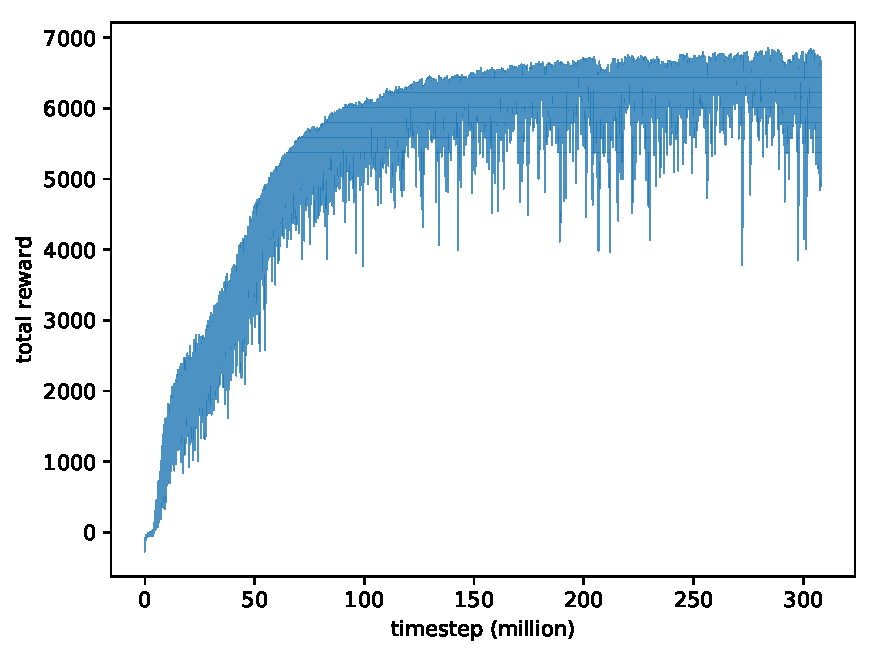
\includegraphics[width=0.7\textwidth]{rec_180608_wass_decay}
	\centering
	\caption{Performance of a W-KTR agent with a decaying W2-metric from 0.02 to 0.00003 in the first 15 million time-steps. The agent is trained with batch-size 4000 and 20 parallel agents. The vertical axis is the total return averaged over the recent 20 episodes and the horizontal axis is the number of million time-steps}\label{fig_wass_decay}
\end{figure}

The experiment results show that the proposed W-KTR algorithm is able to achieve the same level of final performance as the contemporary state-of-art methods. The major drawback is that the algorithm has a long training time due to the slow rate of performance improvement at the early phase. On the contrary, the decaying learning rate feature of KL-divergence based trust region algorithms is able to achieve a good rate of performance improvement in the early phase of training.

The performance of the W-KTR method on several other continuous control environments are shown in Figure \ref{fig:wktr_bench}.
\begin{figure}[!htbp]
	\centering
	\begin{subfigure}[t]{0.4\textwidth}
		\centering
		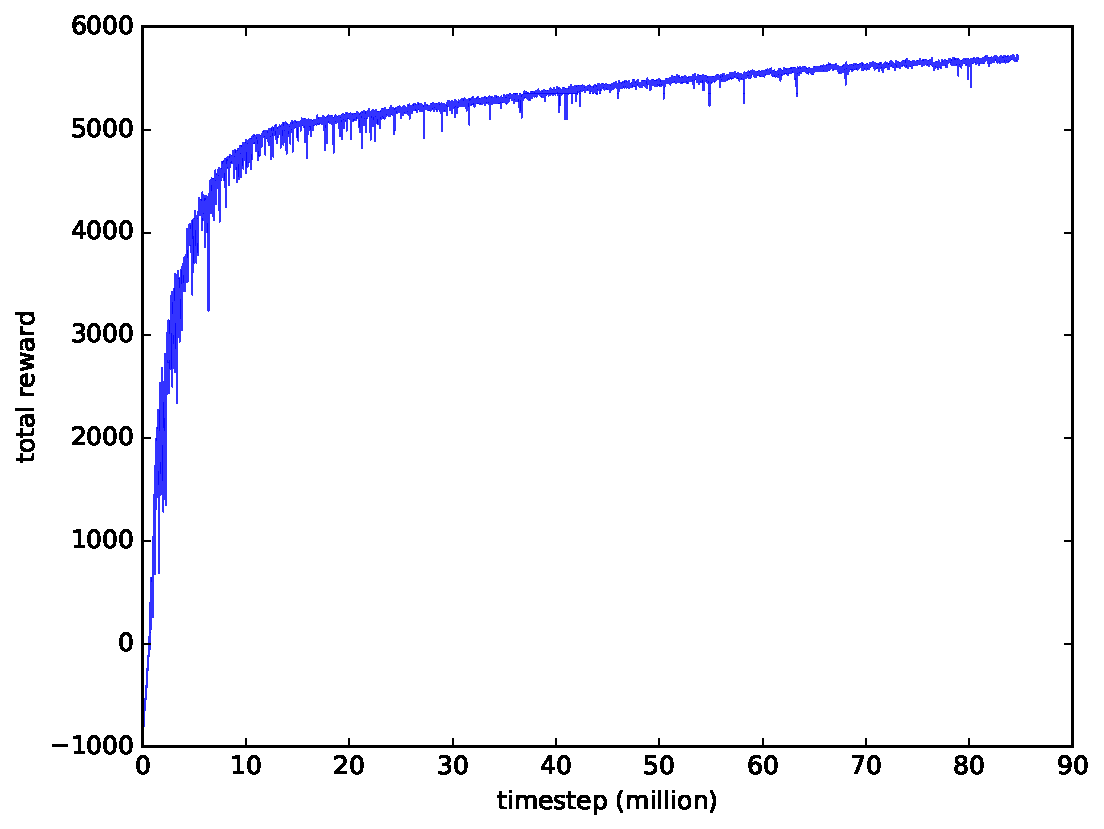
\includegraphics[width=\textwidth]{rec_wktr_halfcheetah}
		\caption{HalfCheetah}
	\end{subfigure}%
	~ 
	\begin{subfigure}[t]{0.4\textwidth}
		\centering
		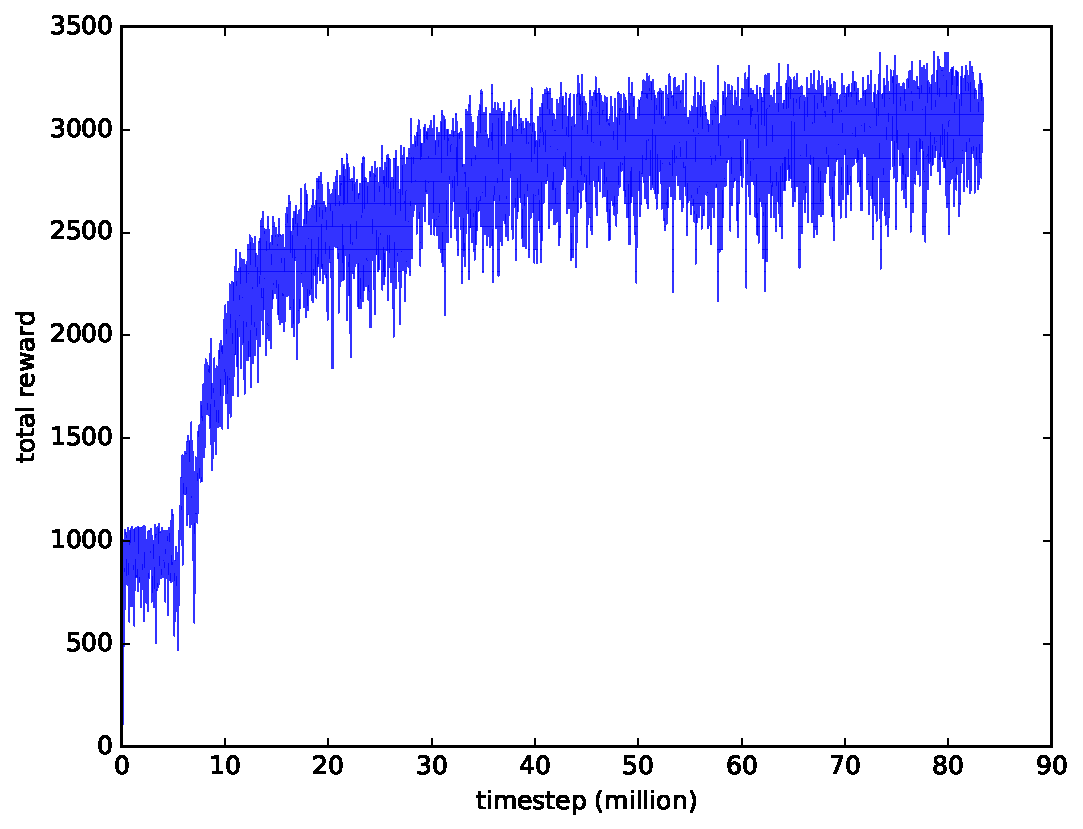
\includegraphics[width=\textwidth]{rec_wktr_hopper}
		\caption{Hopper}
	\end{subfigure}
	~ 
	\begin{subfigure}[t]{0.4\textwidth}
		\centering
		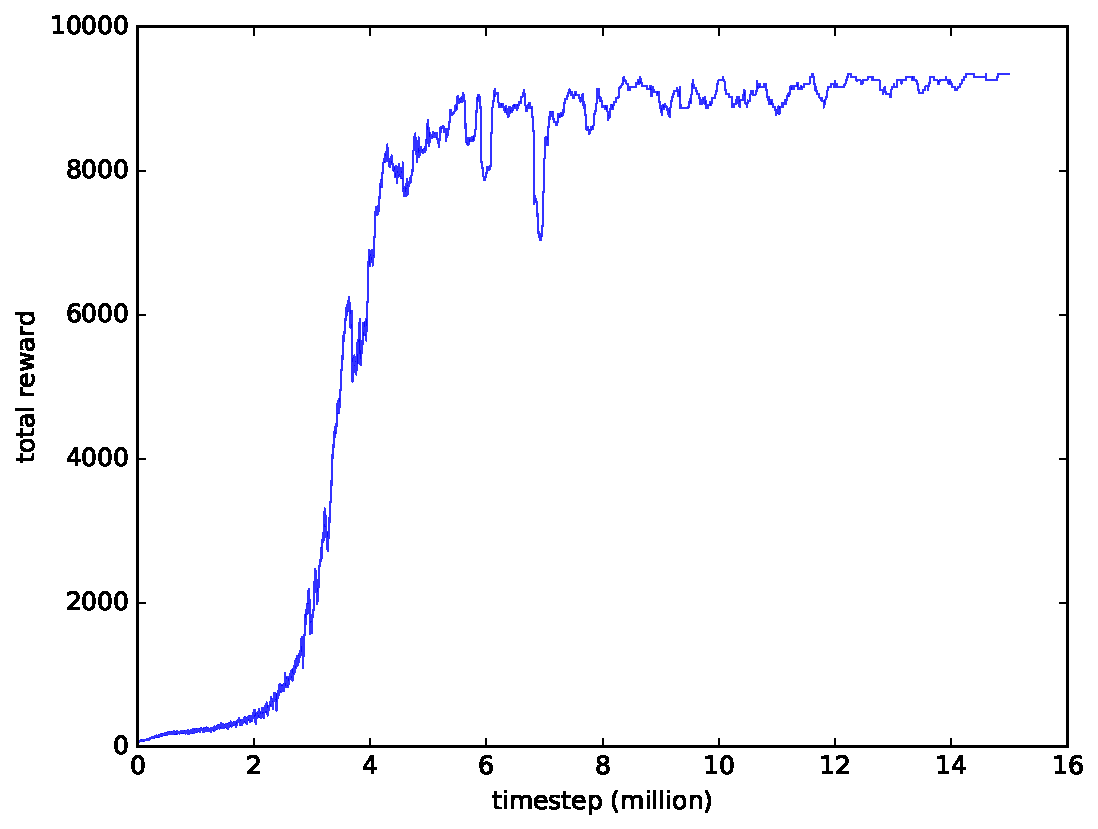
\includegraphics[width=\textwidth]{rec_wktr_inverteddoublependulum}
		\caption{InvertedDoublePendulum}
	\end{subfigure}
	~ 
	\begin{subfigure}[t]{0.4\textwidth}
		\centering
		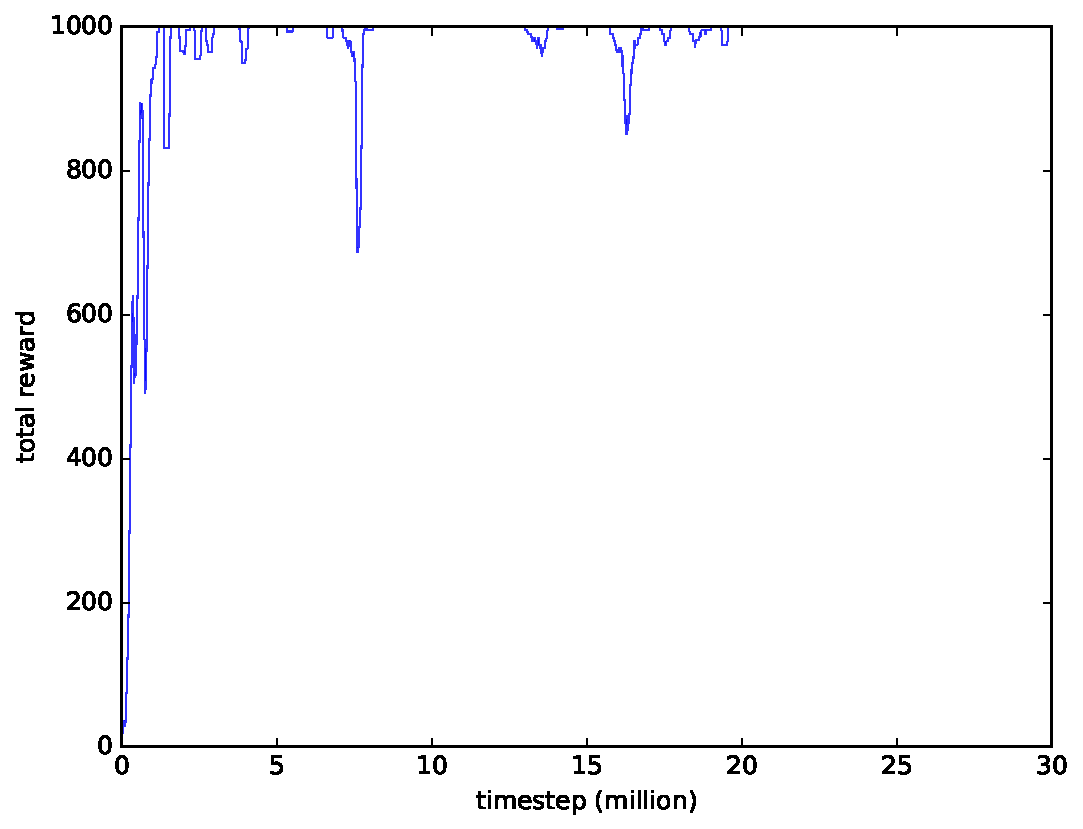
\includegraphics[width=\textwidth]{rec_wktr_invertedpendulum}
		\caption{InvertedPendulum}
	\end{subfigure}
	~ 
	\begin{subfigure}[t]{0.4\textwidth}
		\centering
		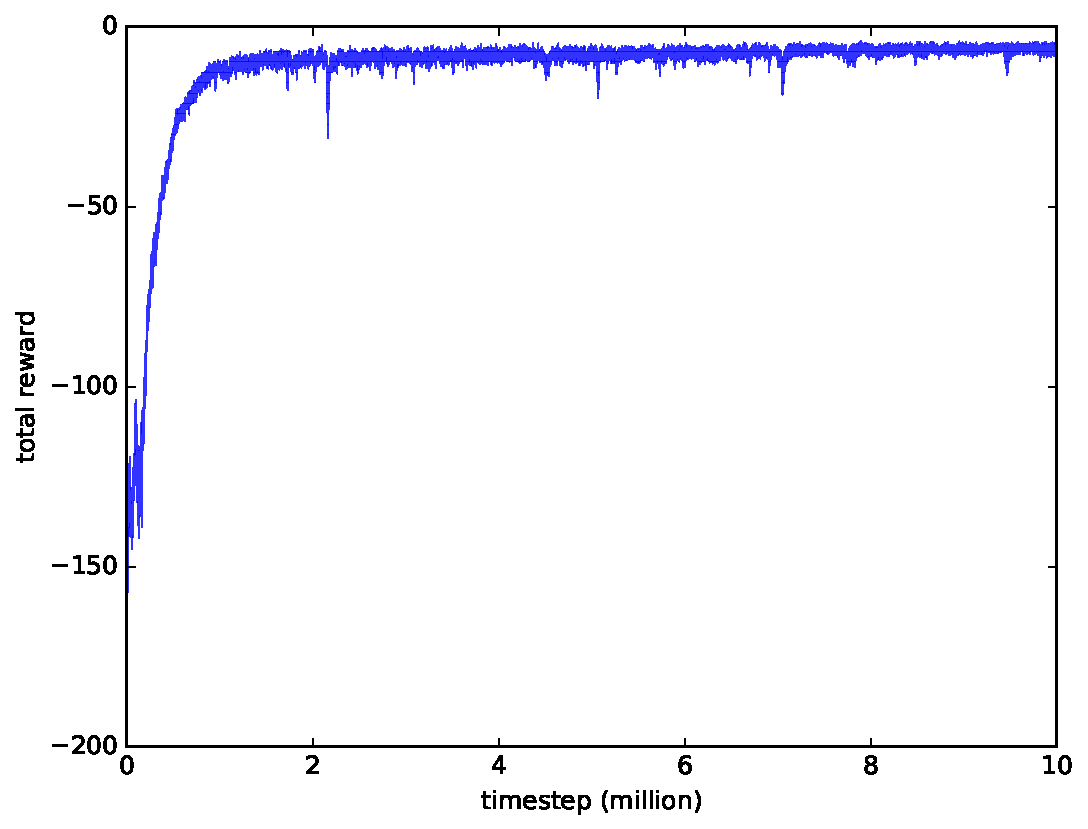
\includegraphics[width=\textwidth]{rec_wktr_reacher}
		\caption{Reacher}
	\end{subfigure}
	~ 
	\begin{subfigure}[t]{0.4\textwidth}
		\centering
		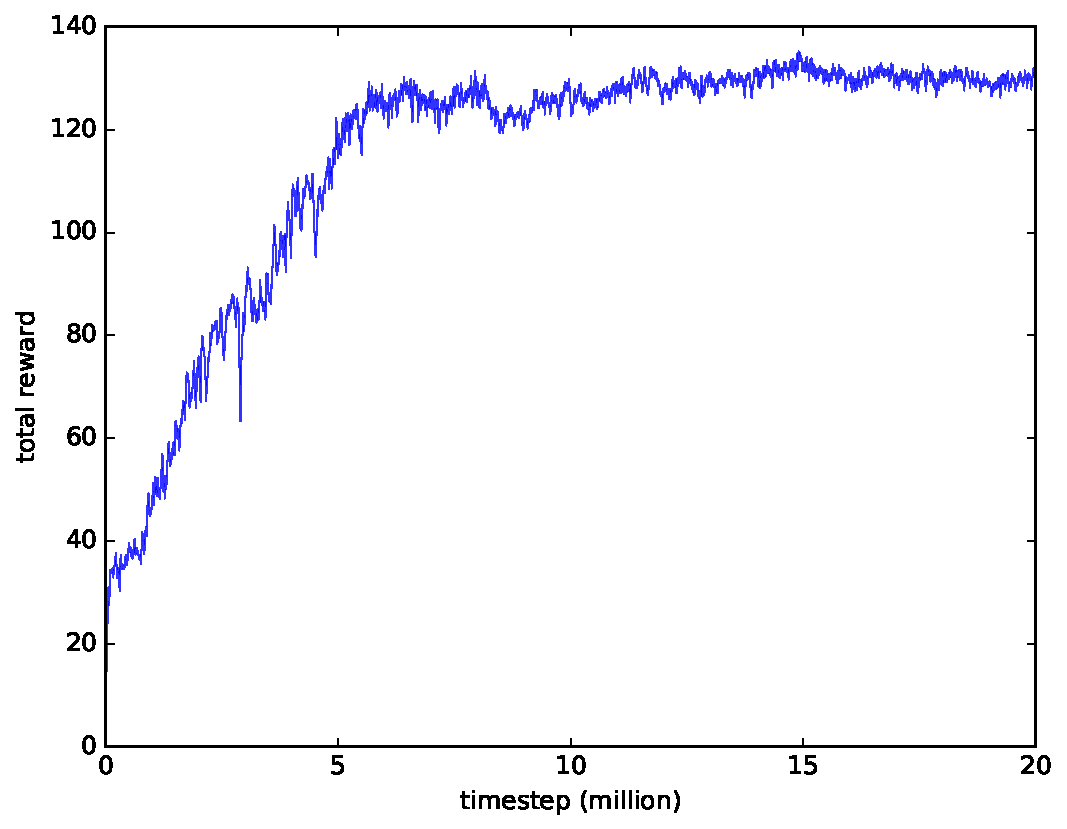
\includegraphics[width=\textwidth]{rec_wktr_swimmer}
		\caption{Swimmer}
	\end{subfigure}
	~ 
	\begin{subfigure}[t]{0.4\textwidth}
		\centering
		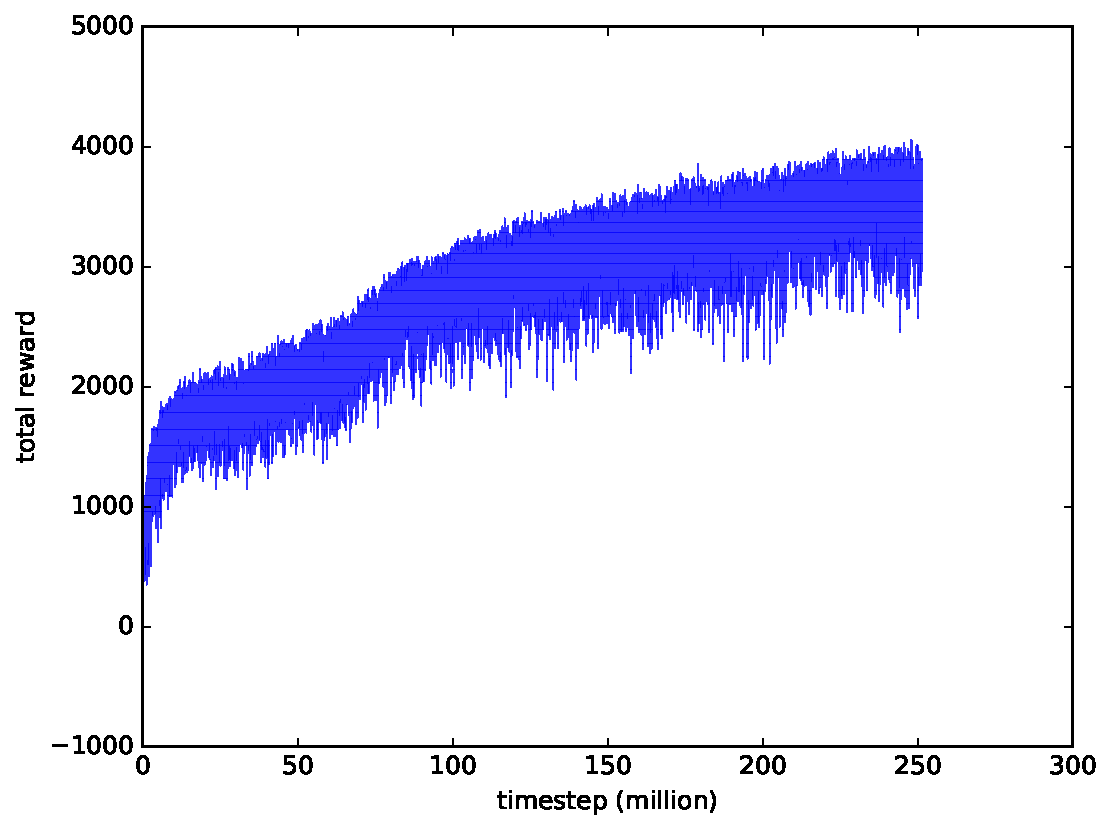
\includegraphics[width=\textwidth]{rec_wktr_walker}
		\caption{Walker}
	\end{subfigure}
	~ 
	\begin{subfigure}[t]{0.4\textwidth}
		\centering
		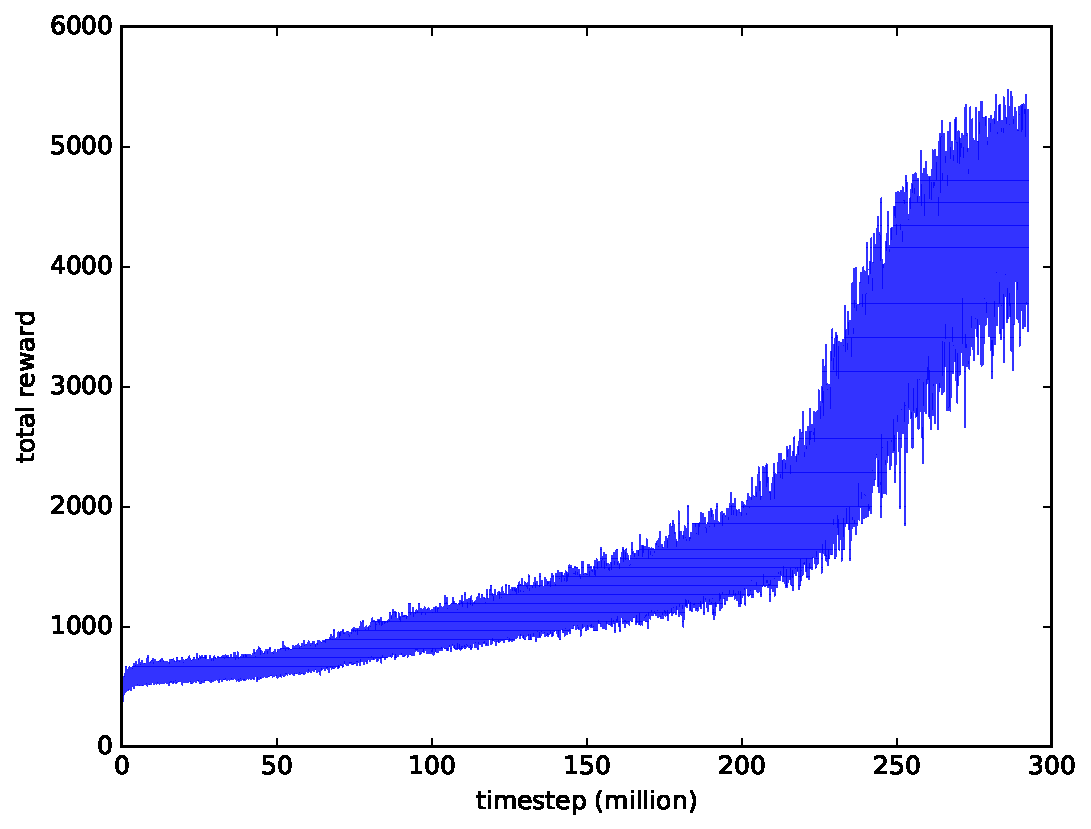
\includegraphics[width=\textwidth]{rec_wktr_humanoid}
		\caption{Humanoid}
	\end{subfigure}

	\caption{The performance of W-KTR on several benchmark environments}
	\label{fig:wktr_bench}
\end{figure}
